\documentclass[article]{jss}
\usepackage[utf8]{inputenc}

\providecommand{\tightlist}{%
  \setlength{\itemsep}{0pt}\setlength{\parskip}{0pt}}

\author{
®yo Lian Hu, ENG\\Coursera / Scibrokes®
}
\title{Odds Modelling and Testing Inefficiency of Sports Bookmakers
\pkg{Rmodel}}
\Keywords{keywords, Bivariate poisson, Multivariate discrete model, Betting strategy, Soccer, English Premier League, Expected return, Maximum likelihood, Statistical forecast, Bookmakers, \proglang{R}, \proglang{Excel}}

\Abstract{
In this paper I am applied a diagonal inflated biviriate poisson as well
as a simple staking model whereby evaluate the efficiency of odds price
offered by 29 sports bookmakers. Finally I get a breakdown profit \&
lose table. While I used Kelly model next to this research which
generated a profit every year.
}

\Plainauthor{®yo Lian Hu, ENG}
\Plaintitle{Odds Modelling and Testing Inefficiency of Sports Bookmakers}
\Shorttitle{\pkg{Rmodel}: Odds Modelling and Testing Inefficiency of Sports
Bookmakers}
\Plainkeywords{keywords, Bivariate poisson, Multivariate discrete model, Betting strategy, Soccer, English Premier League, Expected return, Maximum likelihood, Statistical forecast, Bookmakers, R, Excel}

%% publication information
%% \Volume{50}
%% \Issue{9}
%% \Month{June}
%% \Year{2012}
\Submitdate{}
%% \Acceptdate{2012-06-04}

\Address{
    ®yo Lian Hu, ENG\\
  Coursera / Scibrokes®\\
  09-11-02, Block Chengal, Taman Desaminium, 43300 Seri Kembangan,
  Selangor, Malaysia.\\
  E-mail: \href{mailto:englianhu@gmail.com}{\nolinkurl{englianhu@gmail.com}} /
\href{mailto:englianhu@scibrokes.com}{\nolinkurl{englianhu@scibrokes.com}},
+6017-2100905\\
  URL: \url{https://github.com/scibrokes/owner}\\~\\
  }

\usepackage{amsmath}

\begin{document}

\section{Introduction}\label{introduction}

The odds modelling in Europe and United States are very popular since
decades. However statistical odds modelling and algorithmic staking has
not yet popular in Far East Asia. \bigbreak
  By refer to \emph{Dixon \& Coles 1996}\footnote{Refer to reference
  paper 02}, \emph{Karlis \& Ntzoufras 2005}\footnote{Refer to reference
  paper 08} and also \emph{Dixon \& Pope 2004}\footnote{Refer to
  reference paper 05} I tried to collect soccer data from year 2006 to
2011. The purpose of the research is testing the inefficiency of soccer
odds offered by 29 bookmakers as well as making profit from bookmakers.
\bigbreak
  The paper \emph{Dixon \& Coles 1996} inspired by the \emph{Maher
1982}\footnote{Refer to reference paper 01} to identify the offence and
defence index of every single team where \emph{Karlis \& Ntzoufras 2005}
enahanced to be more complicated model. \emph{Moya 2012}\footnote{Refer
  to reference paper 10} taken 40000 customers' data from bwin to
analayse and profit and lose and applied diversified staking strategies
to make profit from bookmakers. \emph{Goddard 2004}\footnote{Refer to
  reference paper 09} model an ordered probit regression and placed
stkes on English soccer leagues from 1998 to 2002 and finally yeild
\texttt{1998/99} = 0.116, \texttt{1999/00} = 0.008, \texttt{2000/01} =
-0.008, \texttt{2001/02} = 0.160. \bigbreak
  Well, \emph{Dixon \& Robinson 1997}\footnote{Refer to reference paper
  03} has built a rebirth model on 90 minutes In-Play soccer gaming.
\emph{Crowder, Dixon, Anthony \& Robinson 2001}\footnote{Refer to
  reference paper 04} applied MCMC\footnote{Markov Chain Monte Carlo
  model} model for soccer result prediction and do a comparison with
previous \emph{Dixon \& Coles 1996} model where concludes that previous
model forecast more precisely. \bigbreak
  Similar with \emph{Dixon \& Coles 1996}, \emph{Karlis \& Ntzuofras
1998}\footnote{Refer to reference paper 06} has encountered an issue
which is a number of nil-nil tied games. while \emph{Dixon \& Coles
1996} applied an inflation on low scores games while \emph{Karlis \&
Ntzoufras 2005} built an extra distribution parameter to settle it.
\bigbreak
  The latest research paper wrote by Dixon is that \emph{Dixon \& Pope
2004} which have reviewed the previous model and testing the efficiency
on correct score of 3 major firms in UK. \emph{Karlis \& Ntzuofras 2007}
make a summary of evolution on his research which is apply Skellam's
distribution on bivariate poisson model to resolve the obstacle of draw
games. \bigbreak
  Section 2 discribe a statiscal model applicable to soccer odds
modelling. Section 3 talk about the dataset while section 4 model focus
on staking model. Section 5 present the result and last section
conclude.

\subsection{Code formatting}\label{code-formatting}

Don't use markdown, instead use the more precise latex commands:

\begin{itemize}
\tightlist
\item
  \proglang{Java}
\item
  \pkg{plyr}
\item
  \code{print("1+2")}
\end{itemize}

\section{Modelling}\label{modelling}

\subsection{Basic Model}\label{basic-model}

As mentioned in \emph{Karlis \& Ntzuofras 2005}, bivariate Poisson
models are appropriate for modeling paired count data exhibiting
correlation. Paired count data arise in a wide context including:

\begin{itemize}
\tightlist
\item
  marketing (number of purchases of different products)
\item
  epidemiology (incidents of different diseases in a series of
  districts)
\item
  accident analysis (number of accidents in a site before and after
  infrastructure changes)
\item
  medical research (the number of seizures before and after treatment)
\item
  sports (the number of goals scored by each one of the two opponent
  teams in soccer)
\item
  econometrics (number of voluntary and involuntary job changes)
\end{itemize}

Where I just to name a few among the use. \bigbreak

\textbf{Bivariate Poisson regression models}

\begin{figure}[htbp]
\centering
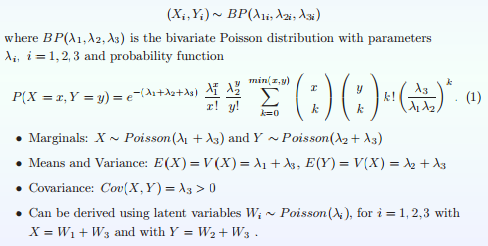
\includegraphics{https://github.com/scibrokes/odds-modelling-and-testing-inefficiency-of-sports-bookmakers/blob/master/figure/1-bp.png?raw=true}
\caption{Bivariate Poisson regression models}
\end{figure}

From above formula, bivariate poisson basically measure the
correlationship between \emph{X} and \emph{Y} compare to double poisson
models. However, as I mentioned which is \emph{Dixon \& Coles 1996}
modified a little on the score 0-0, 1-0, 1-1 and vice versa. \bigbreak

\begin{figure}[htbp]
\centering
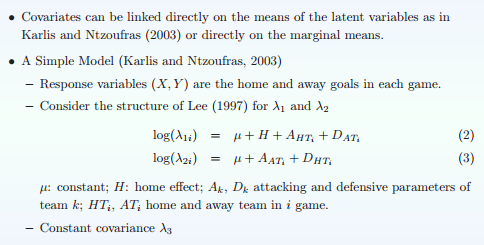
\includegraphics{https://github.com/scibrokes/odds-modelling-and-testing-inefficiency-of-sports-bookmakers/blob/master/figure/2-cov.png?raw=true}
\caption{Double Poisson regression models}
\end{figure}

A Double poisson model can be easily applied by generalized linear
model. The covariates is a constant parameter across all soccer matches
or teams as we know from figure 2. \bigbreak

\textbf{Diagonal Inflated Bivariate Poisson regression models}

\begin{figure}[htbp]
\centering
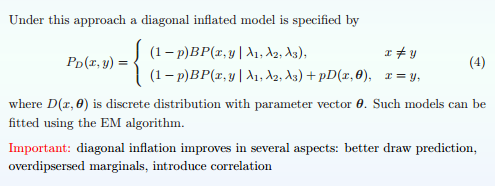
\includegraphics{https://github.com/scibrokes/odds-modelling-and-testing-inefficiency-of-sports-bookmakers/blob/master/figure/3-dbp.png?raw=true}
\caption{Diagonal Inflated Bivariate Poisson regression models}
\end{figure}

Since the bivariate is not accurate enough and applicable to predict the
real life soccer result. \emph{Karlis \& Ntzuofras 2005} introduced a
more complicated model which able to inflated the probabilities of the
occurrance on draw games.

\begin{figure}[htbp]
\centering
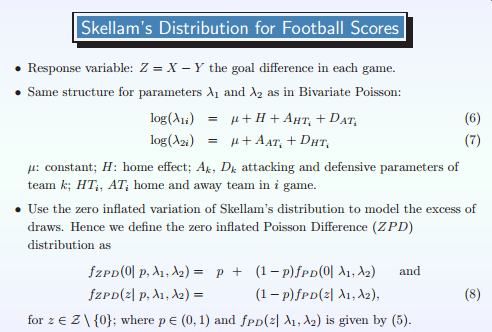
\includegraphics{https://github.com/scibrokes/odds-modelling-and-testing-inefficiency-of-sports-bookmakers/blob/master/figure/4-sd.png?raw=true}
\caption{Skellam's Distribution for Football Scores}
\end{figure}

Well, when we talk about the parameter to measure the correlationship.
How can we know what models might fit into it? \emph{Karlis \& Ntzuofras
2005} has compare few models which are :

\begin{itemize}
\tightlist
\item
  Discrete distribution (with an adjustable paramters)
\item
  Poisson distribution
\item
  Geometric distribution
\end{itemize}

They built 12 statistical models to compare and get the best fit model.
For more details kindly refer to the paper.

\hypertarget{model-enhancement}{\subsection{Model
Enhancement}\label{model-enhancement}}

There has a popular quote in sportsbook betting industry which is term
as \texttt{FORM}. There is a flutuation of the ability and aggresiveness
on sports competition as time goes by. Lets review the \emph{Dixon \&
Coles 1996} model and fit the decay parameter into our basic model.
\bigbreak

\begin{figure}[htbp]
\centering
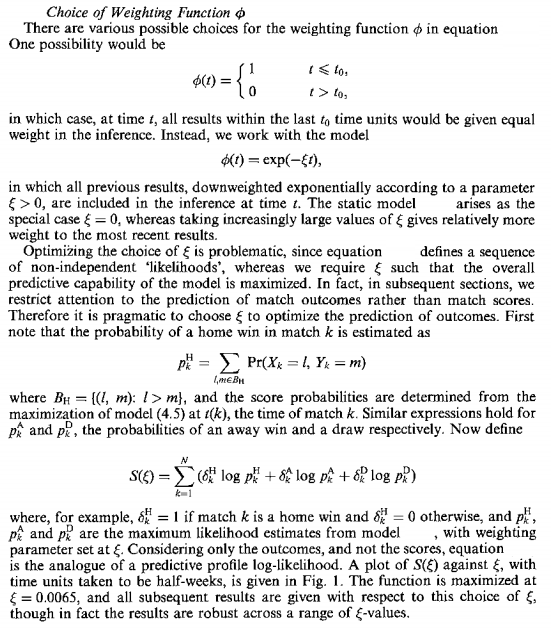
\includegraphics{https://github.com/scibrokes/odds-modelling-and-testing-inefficiency-of-sports-bookmakers/blob/master/figure/5-df.png?raw=true}
\caption{decay rates}
\end{figure}

After simulation, I get a decay rate which is almost \texttt{0.0065} and
similar with \emph{Dixon \& Coles 1996}. However, due to I consider the
soccer matches has come out result once the whistle is blew. Therefore
I've tried to build another model which is similar with Weibull model to
make the decay rate flexible compare to constantly annum. few models,
which are:

\begin{itemize}
\tightlist
\item
  Count in the soccer result once a soccer match is finished to get a
  dynamic decay rates.
\item
  Follow \emph{Dixon \& Coles 1996} which taken a constant decay rates
  for a soccer session.
\end{itemize}

I got a vector of decay rates around \texttt{0.0045} with the standard
deviation not more than 1\textasciitilde{}10\%. which is similar with
the model at \href{http://matchodds.org}{MatchOdds.org}.

\section{Data}\label{data}

\subsection{Soccer Sports Dataset}\label{soccer-sports-dataset}

\subsection{Odds Price Dataset}\label{odds-price-dataset}

I manually copy and paste the odds price from \href{}{500Wan.com}. You
are feel free to browse over the dataset via
\href{200611\%20EngAllOdds}{200611 EngAllOdds}\footnote{The spreadsheet
  file locate inside my previous project which is
  \href{https://www.dropbox.com/home/Research\%20Project\%202}{\textbf{Odds
  Modelling and Testing Inefficiency of Sports-Bookmakers}
  \emph{2008-2010 by ®yo Eng Lian Hu}}.}

\section{Staking Model}\label{staking-model}

\subsection{Betting Strategies}\label{betting-strategies}

As I mentioned in section \protect\hyperlink{model-enhancement}{Model
Enhancement} on the decay rates. In order to test the efficiency and the
return of investment, I've taken both models in algorithmic simulations.

\subsection{Preview of Returns.}\label{preview-of-returns.}

\section{Conclusion}\label{conclusion}

\subsection{Conclusion}\label{conclusion-1}

\subsection{Future Works}\label{future-works}

\section{Appendices}\label{appendices}

\subsection{Documenting File Creation}\label{documenting-file-creation}

It's useful to record some information about how your file was created.

\begin{itemize}
\tightlist
\item
  File creation date: 2016-05-06
\item
  R version 3.2.3 (2015-12-10)
\item
  R version (short form): 3.2.3
\item
  \href{https://github.com/rstudio/rticles}{\textbf{rticles} package}
  version: 0.2
\item
  File version: 1.0.0
\item
  File latest updated date: 2016-05-05
\item
  Author Profile:
  \href{https://beta.rstudioconnect.com/englianhu/ryo-eng/}{®yo, Eng
  Lian Hu}
\item
  GitHub:
  \href{https://github.com/scibrokes/odds-modelling-and-testing-inefficiency-of-sports-bookmakers}{Source
  Code}
\item
  Additional session information
\end{itemize}

{[}1{]} ``2016-05-05 14:17:04 EDT'' setting value\\
 version R version 3.2.3 (2015-12-10) system x86\_64, linux-gnu\\
 ui X11\\
 language (EN)\\
 collate en\_US.UTF-8\\
 tz America/New\_York\\
 date 2016-05-05\\
 sysname release ``Linux'' ``3.10.0-229.20.1.el7.x86\_64'' version
nodename ``\#1 SMP Tue Nov 3 19:10:07 UTC 2015'' ``scibrokes'' machine
login ``x86\_64'' ``unknown'' user effective\_user ``ryoeng'' ``ryoeng''

\subsection{Speech and Blooper}\label{speech-and-blooper}

Firstly I do appreciate those who shade me a light on my research.
Meanwhile I do happy and learn from the research. I do appreciated to
take some spared time to write this thesis where the research has start
from 2008 and finish in 2012. Infact I've finished my research on 2010
before I wrote a proposal to acquire the
\href{http://www.ladbrokesplc.com/}{Ladbrokes}\footnote{Ladbrokes is a
  world leader in the betting and gaming industry with over 2,700
  betting outlets in the UK, Ireland, Belgium and Spain and over 800,000
  active online customers. British public listed company which in the
  Fortune 500 and over hundred years business group.} trading and hedge
fund project in Scicom (MSC) Bhd and extended dataset soccer matches
until 2012. Unfortunately the project has closed but I keep up learning
journey to run my own company
\href{https://github.com/scibrokes/owner}{Scibrokes}\footnote{A
  registered company but not yet in operation. A prospective statistical
  hedge fund company.} some other days. I'll started work as customer
service executive but in somewhere else next week, I am currently
studying distance course data science at
\href{http://www.coursera.org}{Coursera.org}. You are feel free to
browse over my CV at
\href{https://beta.rstudioconnect.com/englianhu/ryo-eng/}{®yo Eng Lian
Hu}. \bigbreak
  I started my research journey when I decided to resign from Caspo Inc.
to be an customer service operator in Scicom (MSC) Bhd. I've search,
collected and read through thousands of research papers to get the
applicable model in our real life investment. Fortunately I found and
know a person
\href{https://englianhu.wordpress.com/sportsbook/boffins-vs-bookies-the-man-who-broke-the-world-leading-bookmakers/}{Boffins
-vs- Bookies (The Man Who Broke the World Leading Bookmakers)} and start
my learning from an outsider which don't know any statistical tools for
modelling until successfully completed the research in year 2012. Kindly
refer to \href{https://englianhu.wordpress.com/}{My personal WordPress
blog} for more experience and bloopers. \bigbreak
  Now I would like to share some bloopers during process this thesis.

\begin{itemize}
\tightlist
\item
  \textbf{Remarks} : Due to the mathematical LaTeX formula and greek
  letters unable use in
  \href{https://github.com/rstudio/rticles}{\textbf{rticles} package}.
  Here I forced to use some image for substitution.
\item
  Due to the Microsoft Excel file inside my previous project
  \href{https://www.dropbox.com/home/Research\%20Project\%202}{\textbf{Odds
  Modelling and Testing Inefficiency of Sports-Bookmakers}
  \emph{2008-2010 by ®yo Eng Lian Hu}} is very huge. I tried to convert
  it to pdf format and attached as appendices but system keep endless
  processing there but no outcome. Secondly, huge dataset make it
  trouble to read into ®Studio and summarise and plotting.
\end{itemize}

\subsection{Reference}\label{reference}

\begin{enumerate}
\def\labelenumi{\arabic{enumi}.}
\tightlist
\item
  \href{https://github.com/scibrokes/odds-modelling-and-testing-inefficiency-of-sports-bookmakers/blob/master/reference/Maher1982.pdf}{\textbf{Modelling
  association football scores} \emph{1982 by M.J Maher}}
\item
  \href{https://github.com/scibrokes/odds-modelling-and-testing-inefficiency-of-sports-bookmakers/blob/master/reference/DixonColes1996.pdf}{\textbf{Modelling
  Association Football Scores and Inefficiencies in the Football Betting
  Market.} \emph{1996 by Mark Dixon and Stuart Coles}}
\item
  \href{https://github.com/scibrokes/odds-modelling-and-testing-inefficiency-of-sports-bookmakers/blob/master/reference/DixonRobinson1997.pdf}{\textbf{A
  Birth Process Model for Association Football Matches.} \emph{1997 by
  Mark Dixon and Michael Robinson}}
\item
  \href{https://github.com/scibrokes/odds-modelling-and-testing-inefficiency-of-sports-bookmakers/blob/master/reference/DixonLedfordRobinson2001.pdf}{\textbf{Dynamic
  Modelling and Prediction of English Football League Matches for
  Betting.} \emph{2002 by Martin Crowder, Mark Dixon, Anthony Ledford
  and Mike Robinson}}
\item
  \href{https://github.com/scibrokes/odds-modelling-and-testing-inefficiency-of-sports-bookmakers/blob/master/reference/DixonPope2004.pdf}{\textbf{The
  value of statistical forecasts in the UK association football betting
  market.} \emph{2004 by Mark Dixon and Peter Pope}}
\item
  \href{https://github.com/scibrokes/odds-modelling-and-testing-inefficiency-of-sports-bookmakers/blob/master/reference/KarlisNtzoufras1998.pdf}{\textbf{Statistical
  Modelling for Soccer Games: The Greek League.} \emph{1998 by Dimitris
  Karlis and Ioannis Ntzoufras}}
\item
  \href{https://github.com/scibrokes/odds-modelling-and-testing-inefficiency-of-sports-bookmakers/blob/master/reference/KarlisNtzoufras2007.pdf}{\textbf{Bayesian
  modelling of football outcomes (using Skellam's Distribution).}
  \emph{2007 by Dimitris Karlis and Ioannis Ntzoufras}}
\item
  \href{https://github.com/scibrokes/odds-modelling-and-testing-inefficiency-of-sports-bookmakers/blob/master/reference/KarlisNtzoufras2005.pdf}{\textbf{Bivariate
  Poisson and Diagonal Inflated Bivariate Poisson Regression Models in
  R.} \emph{2005 by Dimitris Karlis and Ioannis Ntzoufras}}
\item
  \href{https://github.com/scibrokes/odds-modelling-and-testing-inefficiency-of-sports-bookmakers/blob/master/reference/GoddardAsimakopoulos2004.pdf}{\textbf{John
  Goddard and Ioannis Asimakopoulos} \emph{2004 by John Goddard and
  Ioannis Asimakopoulos}}
\item
  \href{https://github.com/scibrokes/odds-modelling-and-testing-inefficiency-of-sports-bookmakers/blob/master/reference/Moya2012.pdf}{\textbf{Statistical
  Methodology for Profitable Sports Gambling} \emph{2012 by Fabián
  Enrique Moya}}
\end{enumerate}



\end{document}

